\documentclass[]{article}
\usepackage{lmodern}
\usepackage{amssymb,amsmath}
\usepackage{ifxetex,ifluatex}
\usepackage{fixltx2e} % provides \textsubscript
\usepackage{wrapfig}
\usepackage{tcolorbox}
\usepackage{lipsum}

\newenvironment{WrapText}[1][r]
  {\wrapfigure{#1}{0.5\textwidth}\tcolorbox}
  {\endtcolorbox\endwrapfigure}

\newcommand\Text{% some text for the example
tesque cursus luctus mauris. Nulla malesuada porttitor diam. Donec felis erat, congue non, volutpat at, tincidunt tristique, libero. Vivamus viverra fermentum felis. Donec nonummy pellentesque ante. Phasellus adipiscing semper elit. Proin fermentum massa ac quam. Sed diam turpis, molestie vitae, placerat a, molestie nec, leo. Maecenas lacinia. Nam ipsum ligula, eleifend at, accumsan nec, suscipit a, ipsum.}

\ifnum 0\ifxetex 1\fi\ifluatex 1\fi=0 % if pdftex
  \usepackage[T1]{fontenc}
  \usepackage[utf8]{inputenc}
\else % if luatex or xelatex
  \ifxetex
    \usepackage{mathspec}
  \else
    \usepackage{fontspec}
  \fi
  \defaultfontfeatures{Ligatures=TeX,Scale=MatchLowercase}
\fi
% use upquote if available, for straight quotes in verbatim environments
\IfFileExists{upquote.sty}{\usepackage{upquote}}{}
% use microtype if available
\IfFileExists{microtype.sty}{%
\usepackage{microtype}
\UseMicrotypeSet[protrusion]{basicmath} % disable protrusion for tt fonts
}{}
\usepackage[margin=1in]{geometry}
\usepackage[unicode=true]{hyperref}
\hypersetup{
            pdftitle={Probabilistic Scenario-Based Design},
            pdfauthor={Scott Sherwin Farley},
            pdfkeywords={Scenario Based Design, Probability, Data Assimilation, User Centered
Design, User Interface, User Experience, Visualization, Design},
            pdfborder={0 0 0},
            breaklinks=true}
\urlstyle{same}  % don't use monospace font for urls
\usepackage{longtable,booktabs}
\usepackage{graphicx,grffile}
\makeatletter
\def\maxwidth{\ifdim\Gin@nat@width>\linewidth\linewidth\else\Gin@nat@width\fi}
\def\maxheight{\ifdim\Gin@nat@height>\textheight\textheight\else\Gin@nat@height\fi}
\makeatother
% Scale images if necessary, so that they will not overflow the page
% margins by default, and it is still possible to overwrite the defaults
% using explicit options in \includegraphics[width, height, ...]{}
\setkeys{Gin}{width=\maxwidth,height=\maxheight,keepaspectratio}
\IfFileExists{parskip.sty}{%
\usepackage{parskip}
}{% else
\setlength{\parindent}{0pt}
\setlength{\parskip}{6pt plus 2pt minus 1pt}
}
\setlength{\emergencystretch}{3em}  % prevent overfull lines
\providecommand{\tightlist}{%
  \setlength{\itemsep}{0pt}\setlength{\parskip}{0pt}}
\setcounter{secnumdepth}{5}
% Redefines (sub)paragraphs to behave more like sections
\ifx\paragraph\undefined\else
\let\oldparagraph\paragraph
\renewcommand{\paragraph}[1]{\oldparagraph{#1}\mbox{}}
\fi
\ifx\subparagraph\undefined\else
\let\oldsubparagraph\subparagraph
\renewcommand{\subparagraph}[1]{\oldsubparagraph{#1}\mbox{}}
\fi

\title{Probabilistic Scenario-Based Design}
\providecommand{\subtitle}[1]{}
\subtitle{Generating insight from probability-based theoretical user models}
\author{Scott Sherwin Farley}
\date{May 4, 2017}

\begin{document}
\maketitle
\begin{abstract}
Constructing hypothetical scenarios and user narratives is a common
technique for communicating the envisioned user experience (UX) of a
tool. Using this approach, application developers, designers, and
stakeholders rapidly build stories of expected use of a tool that
concretize the intended UX. This design strategy is effective, cheap,
flexible, and simple to implement. However, most narrative scenarios
informal textual or visual sketches, lacking a mathematical basis
suitable for statistical testing and visualization of usage patterns. In
this paper, I introduce a new method, probabilistic scenario-based
design (SBD) for underpinning narrative scenarios with probability
statements. Using this technique, tool developers modify traditional
scenarios to include formal statistical statements that describe the
interactivity and design of each interface component. This approach
offers at least three advantages that complement traditional
scenario-based design approaches. First, it offers the potential for
novel visualizations of usage patterns, both real and hypothetical.
These visualizations provide alternate and more concrete view of the
tool's intended UX. Once an early release of the interface is released,
pSBD can enable formal statistical testing of whether intended usage
patterns conform with patterns expected by the UX designers. Finally,
pSBD provides a mechanism of improving interface interactivity and
design that statistically incorporates both real usage data and designer
intuition by specifying probability distributions that can be used in
data assimilation routines. This process would allow the interface to
adapt to user needs throughout its lifetime while using much less data
than traditional AI-based personalization algorithms. The process of
pSBD and the derived visualizations and analyses are illustrated with a
synthetic example based on a web-based interactive mapping tool. pSBD is
designed to be operationalized as part of the an existing ucer centered
design or scenario based design workflow.
\end{abstract}

{
\setcounter{tocdepth}{3}
\tableofcontents
}
\section{Introduction}\label{introduction}

Powerful, easy-to-use programming frameworks and widespread consumer
access to low-cost, high-speed, internet-enabled computing devices have
resulted in a host of highly interactive, richly-featured applications
on the Web. These apps rely on a two-way communication model that
encourages the production of user-generated content and social
interaction among users. As cloud services gain popularity, these
web-based app distribution is becoming increasingly common. Many common
tasks, including email, word processing, and data analysis are
increasingly done `in the cloud', facilitated through
software-as-a-service (SaaS) that enables synchronous information
retrieval and preference persistence across devices to create a seamless
user experience {[}1--3{]}. Often, these applications serve multiple
user groups, with different interests, motivation, or skills {[}4{]}.
While it is possible to simultaneously support multiple user groups
through carefully engineered design decision, artificial intelligence
(AI) and machine learning (ML) algorithms are often applied to recognize
user actions, identify likely sequences of interactions, recommend
suggested products, and adapt the user interface (UI) to likely
preferences to maintain a positive user experience for all users
{[}5--8{]}.Typically, these approaches improve the tool's UX by exposing
the user to less information and visual stimuli, allowing cognitive
function to become more focused on specific tasks. While AI and ML
personalization and customization approaches are widely-used and
efficient, particularly for large applications with many users, these
techniques have two important drawbacks. First, because they typically
model the user based on the sequence of interactions taken by a user
during an interaction session (i.e., the clickstream) these algorithms
often require large amounts of data from many user sessions {[}9{]}.
Such large amounts of real usage data may not be available for early
stage applications still under active development. Second, AI approaches
do not typically account for expected usage as envisioned by the
application developers and domain experts; rather, user models are
generally constructed from the application's usage data {[}10{]}.
However, in many cases, application designers, developers, domain
experts, and other stakeholder groups go to great lengths to
characterize the user and their expected user experience (UX) with the
interface during a user centered design (UCD) process.

Specifically, application developers often work with a team of designers
and domain experts to develop narrative scenarios about the expected UX
of a tool in a process known as scenario based design (SBD) {[}11,12{]}.
Scenarios provide a common vocabulary for communication between
stakeholders by describing how a user will interact with a tool
{[}13{]}. SBD is used in a wide variety of fields and is not limited to
development of software systems {[}14,15{]}. Within software
development, it is often used to inform the requirements of a proposed
tool during their negotiation and to envision the intended use of the
software by multiple user groups. Scenarios provide a flexible and cheap
method of communicating concrete use cases and have been shown to
improve utility and usefulness of the resulting tool {[}13{]}. By
design, the scenarios produced during SBD are informal {[}11{]}. If a
scenario is formalized, it typically changes in both form and purpose
from an illustrative device for communication to a rigorous document
describing the functional requirements of the proposed tool {[}14{]}.
Requirements documents are often more concerned with the feasibility of
the tool than the utility and usability by the envisioned user. However,
a framework for formalizing scenarios while maintaining the flexibility
and central focus on the user would improve communication among tool
builders by ground discussion with statistical and visual evidence of
differences in UX among scenarios. Moreover, formal scenarios could be
used to inform personalization algorithms, resulting in more efficient
customization.

In the present study, I develop a method, probabilistic scenario based
design (pSBD), for creating formal user scenarios that maintain the
connection to the envisioned users by enhancing traditional SBD
scenarios with probability distributions. In this method, each scenario
consists of probability distributions that describe the interactivity
and design of each proposed interface component, function, or logical
element in the envisioned interface. In a simple case, these
distributions can simply represent the probability that the actor in the
scenario will use a specific component. In more complex cases,
distributions can be specified to describe the dimensions of a
user-configurable layout or the geographic center of a map component,
for example.

By introducing a probability model, pSBD facilitates improved inference
of user interaction patterns, even before the interface has undergone
extensive use. Rather than informally constructed narratives that rely
on relaxed language, pSBD scenarios become suitable for formal
statistical testing of user interaction patterns, distinction between
real usage and envisioned usage, and prediction of success of future
interfaces at a component level. Because the probability model is
developed during the planning and development stages along with the UI,
AI customization systems have data to work with immediately that
formally account for the developers' intuition for how user groups will
interact with a tool.

In the present paper, I describe and illustrated three potential
advantages of a pSBD design approach. First, this method would allow for
novel visualizations techniques capable of showing, in a concise manner,
how UX would differ among target user groups. Second, pSBD enables the
formal statistical testing of interaction with an interface.
Specifically, pSBD allows the testing of if real usage patterns conform
with the expectations of the development team. This could be
particularly useful during design interactions to improve the interface
to meet expectations. Finally, pSBD is amenable to Bayesian data
assimilation, where observations of actual usage can be integrated as
the application is deployed. The interface can then adapt, in an
intelligent way, to reflect both the envisioned usage of the designer
and the real world usage patterns of the target audience. While not as
sophisticated as many of the AI personalization systems currently on the
market pSBD is flexible, inexpensive, and requires relatively little
data.

The balance of this paper proceeds as follows. First, I outline
contemporary techniques in user interface personalization and
recommendation, review pertinent literature on SBD, and discuss existing
methods Bayesian inference and prediction in the design and function of
user interfaces. Second, I describe the method for enhancing narrative
scenarios from SBD with probability distributions. Third, I illustrate
the derived statistics, visualizations, and prediction possible with the
new method using a synthetic case study.

\section{Background and Prior Work}\label{background-and-prior-work}

\subsection{Intelligent User
Interfaces}\label{intelligent-user-interfaces}

Modern web apps help us choose what music to listen to, which roads to
drive on, which friends to talk to, and what products to buy. Well
crafted UIs and efficient UXs instill positive feelingss of success and
competency, receding into the background as users focus on their work,
exploration, or pleasure {[}16{]}. In many sophisticated apps, AI and
user modeling can play important roles in helping the interface to
disappear by intelligently limiting the content to which the user is
exposed. By processing large amounts of historical usage data and
building statistical models of user preference, AI systems can limit
consumer exposure to only items that the user is likely to be interested
in or partially execute tasks the user is likely to wish to accomplish.
These systems are highly profitable, particularly in ecommerce -- by
limiting a customer's exposure to a large catalogue of goods, the system
encourages consumer focus on a profitable task (buying an item) rather
than an enabling task (choosing which item to purchase).

At the heart of many AI personalization algorithms are user models that
describe and quantify the traits of the application users. The
construction of user models is a focus of active research in
contemporary human-computer interaction study, and is important in
recommendation systems, social computing, intelligent search algorithms,
and adaptive interfaces{[}17{]}. Specifically, user modeling involves
inferring unobservable information about the user, such as his or her
thought processes, intentions, etc, from observable information, such as
his/her actions {[}18,19{]}. While user modeling need not be
quantitative, statistical user models allow an application to anticipate
behavior, including goals, actions, and preferences {[}18{]}. Models can
be constructed as top-down, in which a theoretical understanding of user
preferences are prescribed by the model developer, or bottom-up in which
associations between sequences of user actions are learned organically.
However, most contemporary user modeling approaches can be seen as
hybrids that combine aspects of these two categories {[}20{]}.

In addition to generating personalized recommendations, user models can
be used to underpin adaptive user interfaces (AUIs) which adapt in look,
feel, and interactivity to that most likely to be preferable to a new
user, based on their series of actions. AUIs can provide just-in-time
assistance by predicting the user's most likely actions and then
performing one or more of those actions on the user's behalf {[}21{]}.
AUIs can adapt to the needs of different users for a variety of tasks
{[}7{]}. AUIs have commonly been implemented in the context of
intelligent tutoring and online educations systems. In these cases, the
system must adapt to a user's learning syle and pace, and a user model
is used in tracking how the user is progressing towards and educational
goal {[}22,23{]}. Typically, AUIs work by identifying membership in a
user group based on a series of interaction events, which requires
tracking all user interaction sequences {[}21{]}. Moreover, the more
adaptive an interface, the larger the amount and quality of feedback it
needs from users to determine if it is adapting in a favorable way
{[}7{]}.

Multi-level interfaces are an important target for AI assistance.
Multi-level interfaces are specifically designed to support multiple
tasks of increasing difficulty for users of different skill levels,
motivations, or expertise. For example, a novice user could receive a
more detailed and longer sequence of dialog steps than an expert
familiar with the system {[}24{]}. Such systems would identify the
appropriate user model, then assemble the user interface components most
suitable for the identified context of use {[}24{]}.

\subsection{Scenario Based Design}\label{scenario-based-design}

SBD scenarios are flexible, low-cost, and evocative narratives of a
designer's envisioned use for a tool. SBD has been applied to a variety
of context; however, while the details may differ between
implementations of SBD, all are aimed at concretely describing the use
of a tool early in its development {[}25{]}. These narratives generally
contain four elements: (1) a setting, (2) an actor with personal
motivation and skills, (3) assumptions and context about the actors and
their objectives, and (4) sequences of actions and events in which the
actors manipulate the tools and objects surrounding them {[}12,14,26{]}.
Typically, actors execute a sequence of actions and events that lead to
some outcome {[}25{]}. Scenarios can be expressed in a variety of ways,
such as through text, videos, mockups, or storyboards.

It is important to note that scenarios, by design, are informal and do
not attempt to outline the functional requirements of the interface
under development. Scenarios serve as a sketch of the envisioned UX of
the tool, capturing the essence of future uses of the tool {[}26{]},
evoking reflection in the context of design {[}12{]}. Rather than
enumerating requirements, they can be used as a communication tool to
ground conversations about the design and interactivity of the
application. Scenarios can facilitate brainstorming between development
team members, inform UI design choices, and act as a guide when
developing formal requirements {[}13,26{]}. Like other user-centered
design approaches, scenarios maintain a central focus on the target user
of the tool, and are thereby able to effectively communicate tradeoffs
between design decisions for those specific user groups {[}12{]}.
Moreover, the products created during SBD can be used as design
rationale in later phases of the design cycle.

While scenarios provide a clear communication mechanism and concrete
products on which to guide future development and design activities,
they typically lack a mathematical or statistical basis. A previous
attempt to quantify a scenario with a preference matrix was described in
{[}17{]}, but focuses primarily on the affinities of the user, rather
than the attributes of the proposed interface.

\subsection{Bayesian Inference}\label{bayesian-inference}

Bayesian approaches to knowledge representation are common in many
fields, including in user modeling and adaptive user interface design.
Bayesian statistical inference involves drawing concrete conclusions
about unobservable qualities of a system, in the presence of
uncertainty. These claims are represented in terms of probability
statements, conditional on the analyst's belief of the true nature of
the system and the observed dataset {[}27{]}. In classical statistics,
it is difficult to take into account prior knowledge when testing
hypotheses and statistical experiments demand large sample sizes.
Moreover, it is difficult to use the results from one experiment to
predict the outcome of a future experiment {[}28{]}. The Bayesian
paradigm provides a coherent approach for combining information from new
and existing information in a probabilistic framework {[}29{]}. Bayesian
inference allows the a probability model to be fit to a new dataset, and
the results summarized by probability distributions on both the
parameters of the model and unobserved, or unobservable, latent
qualities of a system {[}27{]}. Bayesian inference is often used in the
context of probabilistic forecasting or data assimilation, where an
existing numerical or physical model is used in conjunction with a set
of observations to update knowledge about the true state of a system
{[}29{]}.

Bayesian belief networks (BBNs) are common technique for representing
user models in AI-based personalization systems. Bayesian belief
networks are directed acyclic graphs (DAGs) in which each node
represents a conditional probability of a particular event's occurrence.
The probability that an event will occur can be estimate by traversing
the graph and calculating the conditional probability at a node, given
that all prior events have occurred. BBNs are a powerful structure for
representing knowledge and reasoning about future events under
conditions of uncertainty {[}30{]}. BNN-based user models can take into
account a user's background, actions, and previous search queries when
reasoning about what the user's intention is most likely to be
{[}23,31{]}. BBNs have been used in a variety of contexts related to
user modeling, including in Microsoft Office Assistant {[}23{]},
educational tools and interactive tutoring applications {[}22,23{]}, and
health-related smartphone apps {[}32{]}.

BBNs require that the entire state-space is described, a process that
can be difficult to accomplish manually. Many early AI interfaces relied
on manual specification of all conditional probabilities in the graph,
leading to a bottleneck in which humans were the limiting factor in the
derivation of new knowledge{[}18{]}. In many modern contexts, alternate
techniques are used to build state-space graph and calculate conditional
probabilities, from formal descriptions of expert knowledge {[}22{]} or
by creating them from the underlying user interaction data {[}5,33{]}.

Data assimilation involves fusing observations and prior knowledge
together is a statistical framework to obtain an estimate of the
distribution of the true state of the underlying process {[}29{]}. In a
Bayesian context, this can be accomplished by using Bayes theorem to
obtain a posterior distribution through the use of a likelihood function
and prior function. Data assimilation is often used in a spatiotemporal
context for numerical weather and climate models {[}29,34{]}, as well as
in ecological and phylogenetic modeling {[}35--37{]}, among other
fields.

\section{Method}\label{method}

Underpinning a user-case scenario with probabilities is an iterative
process that may involve designers, developers, and stakeholders. While
it is not essential, it may be helpful to have low-fidelity wireframes
{[}38{]} of the intended interface. These wireframes, rough visual
outlines of the intended tool, can be used to identify, name, and
visualize the components during pSBD negotiations. If statistical
testing and data assimilation is desired, an alpha- or beta- release
prototype of the application capable of capturing use feedback or user
generated configurations, so that real user content can be compared to
the developer's expected use cases.

\subsection{Develop narratives}\label{develop-narratives}

The first step in pSBD is to develop one or more clearly defined
narrative scenarios for the tool's UX. These scenarios should contain
the four essential elements of traditional SBD, namely actions, context,
goals and objects, and actions and events that lead to an outcome
{[}14{]}, to clearly describe the intended usage of the application.
These narratives may be articulated in visual or textual form, according
to the preference of the development team. For reference on building
traditional SBD scenarios, see {[}25{]} and {[}12{]}.

\subsection{Assign probability
statements}\label{assign-probability-statements}

The second, and most fundamental task in pSBD, is to enhance narratives
with probability statements that capture the intuition and intentions of
the application developers. For each scenario, each component of the
intended interface may be enhanced with one or more probability
distributions that describe its interactivity or design. For example,
these statistical descriptions may quantify the probability that a
particular interface component is used, the geographic center of a map
component, the likely value of a numeric filter widget, or the width of
a configurable panel element. In general, the goal of this step is to
characterize the interactivity or style of each component as a random
variable, and specify the expected value, variance, and distribution of
these variables for the actors in each scenario. In this way, a level of
`agency' is allowed within each user model, while characterizing general
differences that delineate distinct user models.

An essential piece of this framework is specifying the correct
distribution to use in the scenario. While any distribution may be used
in this process, several appear particularly useful in the context of
pSBD. Because of interface constraint, users are typically not exposed
to infinite degrees of freedom within an interface. Thus, most
continuous distributions with infinite support may be less appropriate
than discrete distributions and distributions with truncated support
over smaller intervals. The binomial distribution and its special case
the Bernoulli appear to have particularly useful applications in pSBD.
The probability that a certain interface component is used in a given
scenario may be modeled as a Bernoulli distribution, with a single
parameter \(\alpha\) that describes the probability of use in the
scenario. Component dimensions, such as width, can be modeled as a
binomial distribution with 100 trials with an \(\alpha\) probability of
success, corresponding to the expected width in the scenario. The number
of times users invoke a specific feature can be characterized using a
Poisson distribution. While more complex distributions, particularly
continuous distributions, may be helpful in characterizing complex usage
patterns, they have not been tried at the present time.

Because the probability-enhanced scenarios are, like traditional SBD
scenarios, a way to facilitate communication between project
stakeholders, they should be collectively refined by developers,
designers, domain experts, and other stakeholders. During this
processes, the expectation of each distribution may be modified
according to team consensus. In some cases, new distributions may be
proposed to model components in alternate ways, such as modeling an
event as a Poisson distribution rather than a binomial distribution.
This exercise alone may have significant benefit to the development of
the application, as it will provide a common, rigorous ground on which
to negotiate envisioned tool use. To facilitate communication, some of
the visualizations introduced below may be produced on the fly to
dynamically reflect the negotiated product.

Communication and negotiation with the target users can be done in
several ways. Informal interviews with key members of each stakeholder
may be the best approach. Other social science data collection methods,
including formal interviews or focus groups may also be effective. While
an online survey would capture the input of more potential users, it may
be more effective to limit feedback to a few key stakeholders. The input
of real users may be captured through interaction logging and used to
refine the distributions during the data assimilation phase discussion
below.

\subsection{Visualization}\label{visualization}

Once the distributions have been specified and finalized, the resulting
user model is available for visualization and inference. An initial
analysis step is to generate probability probability-generated
configurations (PGCs) by drawing at random from each distribution in the
pSBD scenario. Using a scripting language such as R {[}39{]} or python
{[}40{]} independent draws from a probability distribution with given
parameters can be easily simulated. A PGC is considered complete when
each component distribution has been drawn from. Therefore, a complete
PGC represents an interface configuration representative of the
corresponding scenario. It is useful to draw 100s or 1000s of PCGs for
each scenario, allowing the PGCs to completely represent the
distributions given in pSBD.

A set of complete PGCs can then be used to produce visualizations
regarding component use or design among groups or to highlight
intra-group variability. Density curves, that plot the density of a
parameter distribution, or bar charts, which plot the frequency of
boolean outcome, can be effective in communication and negotiation.
Principle components analysis and its associated plots can be effective
method of succinctly describing multivariate differences among
scenarios, as represented by interface components. Finally, wireframes
with each component overlaid with the corresponding probability density
function, may prove useful in gaining a holistic view of how an
interface might look under multiple scenarios. These visualization are
developed further in the case study below.

\subsection{Integration with real usage
data}\label{integration-with-real-usage-data}

If the application in question does have an early version release ready
for user tests (alpha- or beta- stage), the pSBD scenarios and
observations of real user interactions and configurations may be used in
conjunction to test similarities and refine the existing distributions.
Traditional k-means cluster or fuzzy c-means clusters can be helpful in
determining whether real usage data is likely to be distinctly different
than an existing pSBD scenario. Traditional clustering delineates crisp
boundaries among two or more clusters, while fuzzy c-means uses fuzzy
logic to assign probabilities of membership to each cluster to each
point in a dataset. While both may prove effective, fuzzy c-means is
conceptually more appropriate, as it allows cluster to overlap, as they
might in the real world. For example, a graduate student user may
exhibit characteristics of the pSBD scenarios developed for researcher
and student personas.

Once a clustering method has been selected, a clustering rule, such as
the silhouette method, can be used to assess the optimal amount of
clusters in a dataset. The silhouette method works by quantifying the
agreement within a cluster (cohesion) and different among clusters
(separation){[}41{]}. The silhouette statistic is calculated by taking
the difference between the cohesion coefficient and the separation
coefficient. For a given \(k\) clusters, the closer this statistic is to
1, the better the points are clusters. The optimal number of clusters --
that which maximizes within cluster homogeneity while maximizes between
cluster variance -- can be found by trying different values of \(k\),
and selecting the \(k\) with the highest average silhouette statistic
value.

\subsection{Data assimilation}\label{data-assimilation}

Real usage patterns can alos be assimilated into the existing pSBD
distributions using Bayes' Theorem to provide an updated estimate of the
human patterns of interaction with the interface. Formally, Bayes
Theorem \(P(\theta \vert y) \propto P(y \vert \theta)P(\theta)\), states
that the posterior distribution of a parameter (\(P(\theta \vert y)\))
is proportional to a likelihood function (\(P(y \vert \theta)\)) times
the prior distribution of the parameter (\(P(\theta)\)). In other words,
the posterior distribution, which quantifies updated inference about the
unobservable parameter's distribution, is related to the likelihood of
the observed data, given the model, and the analyst's prior knowledge
about the parameter's distribution. As additional data become available,
the theorem can be applied an arbitrary number of times; in each
successive iteration the posterior becomes the prior, representing the
current knowledge of the users' activities.

To apply Bayes' Theorem, both a prior and likelihood distribution are
required. During the pSBD design process, information sufficient for
forming the prior distribution was given, making this process relatively
easy, particularly if conjugate prior distributions are chosen. A
conjugate prior function is one that results in a posterior of the same
family (e.g., exponential), and their use allows Bayes' theorem to be
solved analytically in closed-form. While nonconjugate priors do not
pose a structural problem in the analysis, they can hinder direct
interpretation {[}27{]} and often require a numerical solution using
complex sampling algorithms such as the Gibbs sampling and Markov Chain
Monte Carlo (MCMC) integration {[}42{]}. The details of an analytical
application of Bayes' Theorem to a beta prior and binomial likelihood is
shown in Box 1.

\begin{WrapText}
\Text
\end{WrapText}

In the context of pSBD, a common conjugate prior is the beta
distribution, as it provides an easily-interpretable,
analytically-tractable prior distribution for the probability of success
parameter in the binomial distribution. As the prior to a
binomially-distributed likelihood in a data assimilation context, the
Beta prior represents current knowledge about how the probability of
success is distributed, with uncertainty. This distribution has two
shape parameters \(\alpha\) and \(\beta\) and has support on the
interval {[}0, 1{]}.\strut


The first step in the assimilation is to choose the appropriate
parameters for the prior distribution. Specifying the shape parameters
of the beta prior may seem arbitrary, so it may be more efficient to
calculate these parameters based on the expected value and effective
sample size of the distribution. Specifically, the expected value of a
beta distribution is given as \(m = \frac{\alpha}{\alpha + \beta}\) and
the effective sample size of the distribution is given as
\(\nu = \alpha + \beta\). Therefore, \(\alpha = \nu * m\) and
\(\beta = \nu(1 - m)\). Thus, it is possible to work in terms that are
directly related to how we expect the random variable to behave and our
current degree of belief in the distribution. Furthermore, by working
with \(\nu\) and \(m\), the terms are more equivalent to parameters of a
beta distribution, making comparisons with the likelihood function
easier. To apply Bayes' theorem, we multiply the likelihood function by
the prior function to obtain the posterior that represents a weighted
combination of the two. If, as above, we assimilate a binomial
likelihood (\(Y\) successes in \(N\) trials) with a beta prior
(\(\alpha\) and \(\beta\)), our posterior distribution shape parameters
are \(\alpha = Y + (n*m) - 1\) and \(\beta= N - Y + (n*(1-m)) - 1\). The
posterior, likelihood, and prior can be effectively visualized using
density curves to illustrate the differences between the
distributions.\textbar{}

\section{Case Study}\label{case-study}

\subsection{Introduction}\label{introduction-1}

In this section, I introduce a simple yet illustrative case study to
demonstrate the process and utility of pSBD. Consider a web-based
interactive application with an interface whose purpose is to support
understanding of the spatiotemporal and multivariate attribute patterns
of crime events in Chicago (loosely based on {[}43{]} and {[}44{]}). The
developers of this application wish to support a rich interactive map,
encouraging users to browse the spatial patterns of crime, while
providing details, including crime type, date and time, for each
incidents on demand.

The proposed interface design includes two components, a central
\emph{main map} container that features a `slippy map' that enables
users to pan and zoom through space, with crime incidents overlaid as
points, symbolized according to incident type. A secondary panel, the
\emph{information panel} provides the additional details about each
individual crime. The contents of the information panel are updated each
time a user clicks on a point symbol in the main map. The information
panel can be resized or closed via user interaction on the corresponding
resize and toggle buttons. If the panel is resized, the panel is dragged
to a width of \(\gamma\%\) and the map is automatically shrunk to
\(100-\gamma\%\). Similarly, it the information panel is closed, the map
is resized to take up 100\% of the page width. The default configuration
is that

The developers of this interface envision two potential user groups,
novices and researchers. A key difference between novices and
researchers is that novices are expected to be unlikely to dig deeply
into the details of each crime. To support a user-centered design
process, the application developers envisioned two simple scenarios to
describe the intended UX of the tool for each of these user groups
(Table 1).

\begin{longtable}[]{@{}c@{}}
\toprule
Table 1: Narrative scenarios\tabularnewline
\midrule
\endhead
\bottomrule
\end{longtable}

\begin{longtable}[]{@{}c@{}}
\toprule
\begin{minipage}[b]{0.97\columnwidth}\centering\strut
Scenario: Novice\strut
\end{minipage}\tabularnewline
\midrule
\endhead
\begin{minipage}[t]{0.97\columnwidth}\centering\strut
\emph{User one is a first-year student at the University of Chicago. She
has a personal motivation to visualize the crime patterns, because she
was born and raised in Chicago. Moreover, in an introductory course, she
has been tasked with identifying one or more interesting patterns in the
distribution of the crimes, worthy of future investigation. With these
priorities, she is unlikely to investigate the details of each crime;
rather, she is more likely to browse the map itself to determine if she
can recognize patterns in the spatial distribution. She is likely to
focus her attention on crimes near the locations in which she lives and
works. }\strut
\end{minipage}\tabularnewline
\bottomrule
\end{longtable}

\begin{longtable}[]{@{}c@{}}
\toprule
\begin{minipage}[b]{0.97\columnwidth}\centering\strut
Scenario: Researcher\strut
\end{minipage}\tabularnewline
\midrule
\endhead
\begin{minipage}[t]{0.97\columnwidth}\centering\strut
\emph{User two is a criminology professor at the University of
California, Berkeley. She is interested in a recent spike in murders in
Chicago she heard about in news sources, and would like to generate new
hypotheses about the method and weapons of murders in the city. As she
lives in California, she is not familiar with the city firsthand, but is
an expert at recognizing spatial patterns in criminal incidents. She is
likely to make extensive use of the attribute data associated with each
crime. Focusing her attention on these attributes will likely cause her
to reduce the size of the map relative to the information panel.}\strut
\end{minipage}\tabularnewline
\bottomrule
\end{longtable}

\subsection{Assigning Probabilities}\label{assigning-probabilities}

Clear differences in the UX are thus expected between the two user
groups. Indeed, it is possible to imagine, from these scenarios, how the
prototypical user in each user group might interact with the tool and
how their interface might be styled and displayed. At this point, it is
possible to develop the pSBD probability statements for each user group.
In this case study, two attributes regarding the interactivity and
design of the interface will be considered. Specifically, the
probability of using the information panel (\emph{p(infoPanel)}) and the
width of the information panel (\emph{width}) will be considered for
each user group (Table 2).

From the scenario, it is possible to infer that the novice user is
unlikely to investigate the attribute data of each individual crime, and
is more likely to use the main map interface for the majority of her
time with the tool. Thus, she is assigned a low \emph{p(infoPanel)}.
Moreover, if the panel is open, it is likely to be rather small in
comparison to the map element, indicating a small panel \emph{width}.
Specifically, the use of the information panel is modeled as the
Bernoulli distribution \(p(infoPanel)=0.25, X \sim Binom(1, 0.25)\), and
the width of the information component as a binomial distribution
\(width = 0.30, X \sim Binom(100, 0.3)\).

In the researcher's case, extensive use of the information panel and its
attribute data is likely. Much of the academic research made possible
from this interface is likely to require an in-depth understanding of
each incident, in addition to its spatial position. Therefore, the
probability of a researcher using the information panel is much higher,
and the use of this component is modeled as
\(p(infoPanel) = 0.9, X \sim B(1, 0.9)\). Moreover, the research using
is likely to dominate the visual layout of the interface with the
information panel component. A statement about the width of the
information panel can be made to reflect this,
\(width=0.65, X \sim B(100, 0.65)\).

\begin{longtable}[]{@{}ccc@{}}
\toprule
Table 2: Probability Statements & &\tabularnewline
\midrule
\endhead
\textbf{Novice} & &\tabularnewline
Parameter & Distribution & Expectation\tabularnewline
info panel & \(X \sim Binom(1, 0.25)\) & 0.25\tabularnewline
width & \(X \sim Binom(100, 0.3)\) & 0.3\tabularnewline
\textbf{Researcher} & &\tabularnewline
Parameter & Distribution & Expectation\tabularnewline
info panel & \(X \sim Binom(1, 0.9)\) & 0.9\tabularnewline
width & \(X \sim Binom(100, 0.65)\) & 0.65\tabularnewline
\bottomrule
\end{longtable}

\subsection{Visualization of intended
UX}\label{visualization-of-intended-ux}

Draws from the distributions in Table 2 are generated using R {[}39{]}.
Specifically, 1000 draws from each distribution are made to yield 1000
complete PGCs for each scenario. The PGCs are then visualized in three
ways. First, the densities of the width of the information panel
interface component are shown for each user scenario (Figure
\ref{densities}). Second, the frequency of each PGC's use of the
information panel is shown, grouped by the scenario from which the PGC
was drawn. These two visualization types are helpful in communicating
the intended UX between design team members. By allowing a concrete
visual representation of how the intended users will interact with the
tool, UX designers can have a more informed and grounded conversation
that does not rely on weak qualitative language like `more' or `less'.
Moreover, these density plots can be produced and updated rapidly,
allowing efficient visualization of the progress of UX negotiations. A
third potential visualization includes the densities of each parameter
overlaid on a copy of the wireframe, allowing interpretation of the
probabilities in conjunction with the visual design of the interface
(Figure \ref{wireframe_pdf}). This composite visualization may be
appropriate for communicating with domain experts and other
stakeholders, as it gives a holistic view of both the intended design
and UX of the tool.

\begin{figure}[htbp]
\centering
\includegraphics[height=3.00000in]{./densities.png}
\caption{A density plot describing expected panel widths from each user
model in the hypothetical case study\label{densities}}
\end{figure}

\begin{figure}[htbp]
\centering
\includegraphics[height=3.00000in]{./barchart.png}
\caption{A barchart showing relative frequency for use of the
information panel in the hypothetical case study \label{densities}}
\end{figure}

\begin{figure}[htbp]
\centering
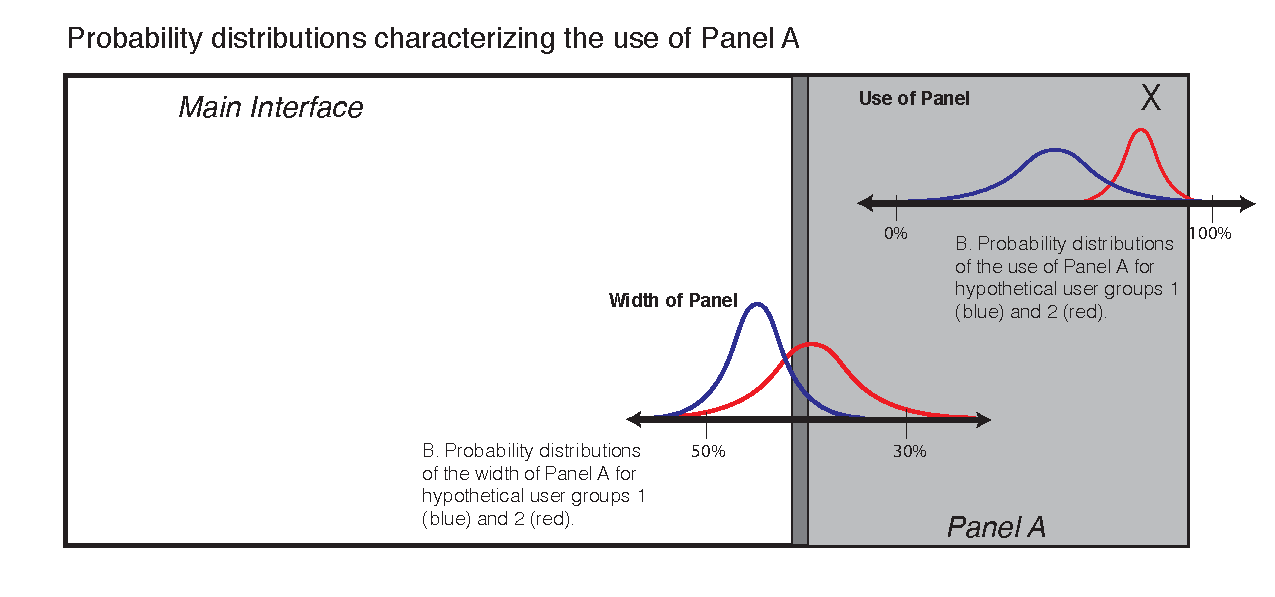
\includegraphics{./fig2_a.pdf}
\caption{PDFs from the pSBD process overlain on top of the low fidelity
wireframe of the interface \label{wireframe_pdf}}
\end{figure}

\subsection{Assessing real usage vs.~expected
usage}\label{assessing-real-usage-vs.expected-usage}

This case study will not examine the process of negotiating the
probability distributions with domain experts and UX designers. Instead,
it will focus on the insights generated by the pSBD process. A
particularly valuable aspect of pSBD is that it can be used to quantify
how real usage differs from expected usage. Typically, this would
require that user actions or configurations are recorded during the use
of an alpha- or beta- stage release of the tool. In this hypothetical
case study, the analysis will be illustrated with a dataset of simulated
observations of real behavior that differ from the scenario models
(Figure \ref{densities_real}).

\begin{figure}[htbp]
\centering
\includegraphics[height=4.00000in]{./densities_w_real.png}
\caption{Densities of panel width with simulated real data included
\label{densities_real}}
\end{figure}

In this case study, a fuzzy c-means algorithm is applied to the
scenario-based PGCs and the simulated real data to determine the optimal
number of clusters in the dataset (\^{}\{C\}). If \^{}\{C\} is two, the
real data falls within the expected usage of one of the two existing
pSBD scenarios. If it is three, the real data is distinct from the
envisioned usage, but forms a coherent cluster. If \^{}\{C\}
\textgreater{} 3, the real data is distinct from the envisioned usage,
but it forms multiple clusters.

The clusters are generated using the \texttt{fanny} function in the R
package \texttt{cluster} {[}45{]}. The silhouette method of choosing the
optimal number of clusters is implemented in the \texttt{silhouette}
function, also in the \texttt{cluster} package. Choices for \(C\)
between 2 and 8 were evaluated, and the \(C\) that maximized the
silhouette statistic was chosen as \^{}\{C\}. In this case, the optimal
number of clusters is 2, indicating that the real usage falls within the
parameters of expected usage envisioned by designers.

\begin{figure}[htbp]
\centering
\includegraphics[height=4.00000in]{./silhouette.png}
\caption{Average silhouette statistic for C=2 to C=8 clusters. Notice
that the maximum silhouette value occurs at \^{}\{C\}=2, indicating an
optimal number of clusters of 2 \label{silhouette_scree}}
\end{figure}

Once the \(C\) is chosen, the degree of membership for each point in the
real and PGC datasets can be visualized in terms of their fuzzy
membership in each cluster(Figure \ref{cluster_contour}). This
visualization shows how the real and PCG data cluster in terms of their
membership in one of two clusters. If the points are clustered in the
top-left and bottom-right of the graph, each point has a high degree of
membership in its respective cluster. If, on the other hand, the points
are clusters in the middle, each point is only a weak member of the
cluster, and has a high similarity with members of other clusters. In
this case, it appears that the novice and research PGC points are
strongly clustered at either end of the membership spectrum and that the
real usage data strongly resembles the envisioned researcher profile. At
this point, the developers may want to reconsider why novice user are
not using the interface in the envisioned way or implement marketing
measures to entice novice users.

\includegraphics[height=4.00000in]{./clusters.png}.

\subsection{Assimilating real usage data into pSBD
scenarios}\label{assimilating-real-usage-data-into-psbd-scenarios}

Finally, the real usage data is integrated with the PGCs using Bayesian
data assimilation to improve the interface's default settings. In this
example, the parameter of interest is the likelihood that a research
user will utilize the information panel. This example will use the same
data as in the previous section, which was concluded to be
representative of academic research use similar to Scenario 2.

Consider a situation in which application developers are weakly
confident in their quantification of the \emph{p(infoPanel)} parameter.
Here, a Beta prior distribution, specified in terms of effective sample
size and expected value, will be used in conjunction with a binomial
likelihood distribution, given as the number of success (uses of the
information panel) and the number of trails (total number of
observations of user behavior). Because the developers are only weakly
confident in their assessment of expected behavior, they may set the
effective sample size of the prior distribution to \(\nu\). This would
correspond to a level of belief in their prior approximately equal to
fifty observations of that behavior. Taking the expectation from Table 2
of \(m=0.9\), the shape parameters of the beta distribution are found to
be \(\alpha=44\) and \(\beta=6\). In the real data described above,
there were 78 uses of the information panel out of a sample of 100
observations of user behavior. The likelihood distribution for this
data, then, is \(X \sim Binom(1, 0.78)\) with 100 independent trials. By
applying Bayes' Theorem, the shape parameters of the posterior
distribution are shown to be \(\alpha = Y + (n*m) - 1 = 122\) and
\(\beta= N - Y + (n*(1-m)) - 1 = 28\). To interpret these new shape
parameters, \(\alpha\) and \(\beta\) can be converted back into terms of
effective sample size and expected value of the posterior distribution.
In this case, the new expected value of the posterior is \(m=0.813\) and
the new effective sample size is \(\nu=150\). Note that this sample size
is the effective sample size of the prior (\(\nu=50\)) plus the number
of observations in the data (\(N=100\)). Moreover, the expectation of
the posterior is a weighted combination of the expected value of the
likelihood (0.78) and the prior (\(0.90\)). Taken together, this
information suggests that a future research has a 81\% chance of using
the information panel (Figure \ref{bayes_1}).

\includegraphics[height=4.00000in]{./weak_posterior.pdf}.

As new observations of the use of the interface are observed via
interaction logging, this data assimilation can be repeated an arbitrary
number of times. Each time, the posterior from the previous iteration of
the assimilation is taken to be the prior for the current iteration.
This new prior distribution is then combined with the new observation to
create a new posterior. For example, if an additional 60 observations of
interface usage are recorded, of which 50 use the information panel,
those observation can be assimilated to obtain new behavior estimates
(\(\alpha=172\), \(\beta=8\), Figure \ref{bayes_2}). The new estimates
forecast that a future user has an 82\% chance of using the information
panel.

\includegraphics[height=4.00000in]{./iter_2_posterior.pdf}.

\section{Discussion}\label{discussion}

\subsection{Advantages of pSBD over traditional
SBD}\label{advantages-of-psbd-over-traditional-sbd}

The hypothetical interface and scenarios described above demonstrate the
visual and analytical power of the pSBD process. One of the most
important advantages of pSBD over traditional SBD is the ability to
rapidly generate visualizations of intended UX for the propose system,
even before a single line of code has been written. Traditional SBD
often uses qualitative language to communicate the differences in usage
between scenarios. By introducing visuals into the design process, pSBD
promotes visual communication to efficient present abstract thoughts and
ideas about the intended UX, replacing the weak language with a visual
model {[}46{]}. Throughout science and industry, tools that support
visual analytics have been a priority in new tool development as a means
to leverage the strengths of both human and computerized data
processing. Broadly, visual analytics tools foster constructive
evaluations, correction, and rapid improvements in our models of
physical processes, and can improve both human knowledge and decisions
{[}47{]}. Visualizations of complex data, such as qualitative,
unstructured descriptions of an intended tool, can offload cognitive
processes to perceptive processes, allowing new features to emerge that
are easily picked up by the visual system {[}48,49{]}. Thus, through the
use of pSBD, designers may uncover unintended patterns that emerge
within and among different use case scenarios.

A second advantage of pSBD is that it allows application designers to
determine if an early stage application is truly serving its target user
groups. Applications that are developed using a user centered approach
typically involve many iterations of feedback from both domain experts
and target users. During this processes, priorities for what the
intended interface should accomplish are identifies. Developers and
designers should ensure that these priorities are actually met by the
delivered application. pSBD allows development team members to assess
whether these development goals are being met, and if not, how the use
of real users differs from the carefully developed expectations.
Moreover, pSBD can be completed with an application very early in the
design process, and does not require the typical, expensive, time
consuming approaches for gathering user feedback traditionally employed
during design iterations, such as interviews, focus groups, or surveys.

pSBD can also be helpful in refining the application's look, feel, and
interactivity on the fly to improve the UX for target user groups. The
interface can be configured to adapt to the updated posterior
distributions to take into account both the developer's intuition and
real observation data on a scenario-by-scenario basis. Effective default
designs for each component are an important part of any interactive
application, and these defaults can be smartly tailored in real time to
the preferences of the application users. If it appears that, contrary
to the developers' expectation, components are used by a majority of the
scenario users, this component can be made to be a default. More
relevant to the design of an application, the width or other aspects of
appearance of a component can be set up to automatically reflect the
expectation of the most recent posterior distribution about that
parameter. Furthermore, this data assimilation technique also allows for
these parameter distributions to change through time. Should user
categories change usage patterns through time, these changes will emerge
from the data. This is an advantage over some AI-based personalization
systems that require an assumption of static preferences through time.

\subsection{Future Research
Priorities}\label{future-research-priorities}

While the current study introduced this technique in a conceptual way
with a hypothetical case study, a forthcoming study will present the
results of a formal implementation of pSBD on a real application.
Several key questions to be addressed in a real application of SBD
include: (1) how accurate are developer's intuitions for the appropriate
scenario probability statements? (2) how are the distributions best
negotiated between developers and stakeholders? and (3) do the
visualizations provided by pSBD positively influence the application
development process? Another worthy research target would be to develop
a Bayesian belief network for each component. As noted above, the
current framework is limited by drawing from independent probability
distributions. If an efficient method for constructing a Bayesian
network of conditional probabilities was developed, pSBD could make
better predictions by conditioning each probability on other components
in the interface.

\section{Conclusion}\label{conclusion}

In this paper, I introduced probabilistic scenario-based design, a new
method for underpinning traditional narrative scenarios during the
development process with statistical distributions. pSBD maintains the
flexibility and low-costs of traditional SBD, but introduces a new set
of visual and statistical tools for application developers to test usage
patterns and assimilate new knowledge. By leveraging Bayesian data
assimilation, the process can formally incorporate developer and
stakeholder intuition with real usage patterns, providing a better
estimate of a latent variable that cannot be observed: human behavior.
Clustering methods can be used to determine whether real usage patterns
fall within existing usage categories, or whether entirely new
categories exist. Several novel visualization types were introduced and
are useful throughout the process for communicating between developers,
stakeholders, and to understand real usage patterns in conjunction with
developer intuition.

\section*{References}\label{references}
\addcontentsline{toc}{section}{References}

\hypertarget{refs}{}
\hypertarget{ref-Hassan:2011uh}{}
{[}1{]} Hassan Q. Demystifying Cloud Computing. CrossTalk 2011:16--21.

\hypertarget{ref-Mosco:2014cu}{}
{[}2{]} Mosco V. To the cloud: Big data in a turbulent world. Routledge;
2015.

\hypertarget{ref-Buyya:2009ix}{}
{[}3{]} Buyya R, Yeo CS, Venugopal S, Broberg J, Brandic I. Cloud
computing and emerging IT platforms: Vision, hype, and reality for
delivering computing as the 5th utility. Future Generation Computer
Systems 2009;25:599--616.
doi:\href{https://doi.org/10.1016/j.future.2008.12.001}{10.1016/j.future.2008.12.001}.

\hypertarget{ref-Roth:2013fv}{}
{[}4{]} Roth RE. Interactive maps: What we know and what we need to
know. Journal of Spatial Information Science 2013:1--57.
doi:\href{https://doi.org/10.5311/josis.2013.6.105}{10.5311/josis.2013.6.105}.

\hypertarget{ref-Adomavicius:2015fx}{}
{[}5{]} Adomavicius G, Tuzhilin A. Context-Aware Recommender Systems.
In:. Recommender systems handbook, Boston, MA: Springer US; 2015, pp.
191--226.
doi:\href{https://doi.org/10.1007/978-1-4899-7637-6_6}{10.1007/978-1-4899-7637-6\_6}.

\hypertarget{ref-Lalle:2015hfa}{}
{[}6{]} Lallé S, Toker D, Conati C, Carenini G. Prediction of Users'
Learning Curves for Adaptation while Using an Information Visualization.
In:. The 20th international conference, New York, New York, USA: ACM
Press; 2015, pp. 357--68.
doi:\href{https://doi.org/10.1145/2678025.2701376}{10.1145/2678025.2701376}.

\hypertarget{ref-Anonymous:VabnjUVa}{}
{[}7{]} Isbell CL, Pierce JS. An IP continuum for adaptive interface
design. Proceedings of HCI International Conference 2005.

\hypertarget{ref-Benson:2010jn}{}
{[}8{]} Benson BJ, Bond BJ, Hamilton MP, Monson RK, Han R. Perspectives
on next-generation technology for environmental sensor networks.
Frontiers in Ecology and the Environment 2010;8:193--200.
doi:\href{https://doi.org/10.1890/080130}{10.1890/080130}.

\hypertarget{ref-linden2003amazon}{}
{[}9{]} Linden G, Smith B, York J. Amazon. com recommendations:
Item-to-item collaborative filtering. IEEE Internet Computing
2003;7:76--80.

\hypertarget{ref-Mulvenna:2000iv}{}
{[}10{]} Mulvenna MD, Anand SS, Büchner AG. Personalization on the Net
using Web mining: introduction. Communications of the ACM
2000;43:122--5.
doi:\href{https://doi.org/10.1145/345124.345165}{10.1145/345124.345165}.

\hypertarget{ref-rosson2009scenario}{}
{[}11{]} Rosson MB, Carroll JM. Scenario based design. Human-Computer
Interaction Boca Raton, FL 2009:145--62.

\hypertarget{ref-Carroll:1999hh}{}
{[}12{]} Carroll JM. Five reasons for scenario-based design. Interacting
with Computers 2000;13:43--60.
doi:\href{https://doi.org/10.1016/S0953-5438(00)00023-0}{10.1016/S0953-5438(00)00023-0}.

\hypertarget{ref-Anonymous:MZBQUkQZ}{}
{[}13{]} Carroll JM, Rosson MB, Chin G, Koenemann J. Requirements
development in scenario-based design. IEEE Transactions on Software
Engineering 1998;24:1156--70.
doi:\href{https://doi.org/10.1109/32.738344}{10.1109/32.738344}.

\hypertarget{ref-mcdonaldm:2004us}{}
{[}14{]} Go K, Carroll JM. The blind men and the elephant: Views of
scenario-based system design. Interactions 2004;11:44--53.
doi:\href{https://doi.org/10.1145/1029036.1029037}{10.1145/1029036.1029037}.

\hypertarget{ref-Anonymous:P3P38N9F}{}
{[}15{]} Kazman R, Abowd G, Bass L, Clements P. Scenario-based analysis
of software architecture. IEEE Software 1996;13:47--55.

\hypertarget{ref-shneiderman2010designing}{}
{[}16{]} Shneiderman B. Designing the user interface: Strategies for
effective human-computer interaction. Pearson Education India; 2010.

\hypertarget{ref-Cunha:2014vu}{}
{[}17{]} Cunha B, Pereira JP, Gomes S, Pereira I, Santos JM. Using
personas for supporting user modeling on scheduling systems. Proceedings
of IEEE HIS; 2014.

\hypertarget{ref-Anonymous:98QvTtXB}{}
{[}18{]} Zukerman I, Albrecht DW. Predictive statistical models for user
modeling. User Modeling and User-Adapted Interaction 2001;11:5--18.

\hypertarget{ref-Young:2010ck}{}
{[}19{]} Young S. Cognitive User Interfaces. IEEE Signal Processing
Magazine 2010;27:128--40.
doi:\href{https://doi.org/10.1109/MSP.2010.935874}{10.1109/MSP.2010.935874}.

\hypertarget{ref-Anonymous:2013be}{}
{[}20{]} Yannakakis GN, Spronck P, Loiacono D, André E. Player modeling
2013;6.

\hypertarget{ref-Anonymous:tFYXZ8fI}{}
{[}21{]} Liu J, Wong CK, Hui KK. An adaptive user interface based on
personalized learning. IEEE Intelligent Systems 2003;18:52--7.

\hypertarget{ref-Anonymous:rA5_Wtin}{}
{[}22{]} Conati C, Gertner A, Vanlehn K. Using Bayesian networks to
manage uncertainty in student modeling. User Modeling and User-Adapted
\ldots{} 2002.

\hypertarget{ref-Anonymous:6QvxqPLs}{}
{[}23{]} Horvitz E, Breese J, Heckerman D, Hovel D, Rommelse K. The
lumiere project: Bayesian user modeling for inferring the goals and
needs of software users. In:. Proceedings of the fourteenth conference
on uncertainty in artificial intelligence, Morgan Kaufmann Publishers
Inc. 1998, pp. 256--65.

\hypertarget{ref-Honold:2014gq}{}
{[}24{]} Honold F, Bercher P, Richter F, Nothdurft F, Geier T, Barth R,
et al. Companion-Technology: Towards User- and Situation-Adaptive
Functionality of Technical Systems. In:. 2014 international conference
on intelligent environments (ie), IEEE; 2014, pp. 378--81.
doi:\href{https://doi.org/10.1109/IE.2014.60}{10.1109/IE.2014.60}.

\hypertarget{ref-Rosson:2002vj}{}
{[}25{]} Rosson MB, Carroll JM. Scenario-based design. In:. The
human-computer interaction handbook, L. Erlbaum Associates Inc. 2002,
pp. 1032--50.

\hypertarget{ref-Rosson:2005vj}{}
{[}26{]} Rosson MB, Carroll JM. Scenario-Based Design. 2005.

\hypertarget{ref-Andrew:2013un}{}
{[}27{]} Gelman A, Carlin JB, Stern HS. Bayesian data analysis 2014;2.

\hypertarget{ref-Ellison:1996js}{}
{[}28{]} Ellison AM. An Introduction to Bayesian Inference for
Ecological Research and Environmental Decision-Making. Ecological
Applications 1996;6:1036--46.
doi:\href{https://doi.org/10.2307/2269588}{10.2307/2269588}.

\hypertarget{ref-Wikle:2007dy}{}
{[}29{]} Wikle CK, Berliner LM. A Bayesian tutorial for data
assimilation. Physica D: Nonlinear Phenomena 2007;230:1--16.
doi:\href{https://doi.org/10.1016/j.physd.2006.09.017}{10.1016/j.physd.2006.09.017}.

\hypertarget{ref-Cheng:1997wg}{}
{[}30{]} Cheng J, Bell DA, Liu W. An algorithm for Bayesian belief
network construction from data. In:. Proceedings of ai \& stat'97, 1997.

\hypertarget{ref-Fischer:2001jl}{}
{[}31{]} Fischer G. User Modeling in Human-Computer Interaction. User
Modeling and User-Adapted Interaction 2001;11:65--86.
doi:\href{https://doi.org/10.1023/A:1011145532042}{10.1023/A:1011145532042}.

\hypertarget{ref-Fan:2015du}{}
{[}32{]} Fan X, Wang J. Bayesheart: A probabilistic approach for robust,
low-latency heart rate monitoring on camera phones. In:. Proceedings of
the 20th international conference on intelligent user interfaces, ACM;
2015, pp. 405--16.

\hypertarget{ref-Anonymous:XBUc-RmI}{}
{[}33{]} Horvitz E. Principles of mixed-initiative user interfaces. ACM;
1999.

\hypertarget{ref-Airoldi:2007br}{}
{[}34{]} Airoldi EM. Getting Started in Probabilistic Graphical Models.
PLoS Computational Biology 2007;3:e252--5.
doi:\href{https://doi.org/10.1371/journal.pcbi.0030252}{10.1371/journal.pcbi.0030252}.

\hypertarget{ref-Dawson:2016wa}{}
{[}35{]} Dawson A, Paciorek CJ, McLachlan JS, Goring S, Williams JW,
Jackson ST. Quantifying pollen-vegetation relationships to reconstruct
ancient forests using 19th-century forest composition and pollen data
2016. doi:\href{https://doi.org/10.1101/039073}{10.1101/039073}.

\hypertarget{ref-Ellison:2004fj}{}
{[}36{]} Ellison AM. Bayesian inference in ecology. Ecology Letters
2004;7:509--20.
doi:\href{https://doi.org/10.1111/j.1461-0248.2004.00603.x}{10.1111/j.1461-0248.2004.00603.x}.

\hypertarget{ref-Ho:2009gn}{}
{[}37{]} Ho SYW, Phillips MJ. Accounting for Calibration Uncertainty in
Phylogenetic Estimation of Evolutionary Divergence Times. Systematic
Biology 2009;58:367--80.
doi:\href{https://doi.org/10.1093/sysbio/syp035}{10.1093/sysbio/syp035}.

\hypertarget{ref-Roth:2015ts}{}
{[}38{]} Roth RE, Hart D, Mead R, Quinn C. Wireframing for Interactive
\& Web-based Geographic Visualization: Designing the NOAA Lake Level
Viewer. Cartography and Geographic Information Science 2015:1--28.
doi:\href{https://doi.org/10.1080/15230406.2016.1171166}{10.1080/15230406.2016.1171166}.

\hypertarget{ref-RSoftware}{}
{[}39{]} R Core Team. R: A language and environment for statistical
computing. Vienna, Austria: R Foundation for Statistical Computing;
2017.

\hypertarget{ref-Rossum:1995:PRM:869369}{}
{[}40{]} Rossum G. Python reference manual. Amsterdam, The Netherlands,
The Netherlands: CWI (Centre for Mathematics; Computer Science); 1995.

\hypertarget{ref-Rousseeuw:1987gv}{}
{[}41{]} Rousseeuw PJ. Silhouettes: a graphical aid to the
interpretation and validation of cluster analysis. Journal of
Computational and Applied Mathematics 1987;20:53--65.
doi:\href{https://doi.org/10.1016/0377-0427(87)90125-7}{10.1016/0377-0427(87)90125-7}.

\hypertarget{ref-Carlin:1991cl}{}
{[}42{]} Carlin BP, Polson NG. Inference for nonconjugate Bayesian
Models using the Gibbs sampler. Canadian Journal of Statistics
1991;19:399--405.
doi:\href{https://doi.org/10.2307/3315430}{10.2307/3315430}.

\hypertarget{ref-chicagoPoliceMap}{}
{[}43{]} Department CP. Clear map crime incidents 2017.
\url{http://gis.chicagopolice.org/clearmap/startpage.htm\#} (accessed
May 6, 2017).

\hypertarget{ref-chicagoShootingsMap}{}
{[}44{]} Ali T. Where shootings have occurred in chicago since 2010
(map) 2016.
\url{https://www.dnainfo.com/chicago/20150707/downtown/where-shootings-have-occurred-chicago-since-2010-map}
(accessed May 6, 2017).

\hypertarget{ref-clusterR}{}
{[}45{]} Maechler M, Rousseeuw P, Struyf A, Hubert M, Hornik K. Cluster:
Cluster analysis basics and extensions. 2016.

\hypertarget{ref-Cyrs:1997gz}{}
{[}46{]} Cyrs TE. Visual Thinking: Let Them See What You Are Saying. New
Directions for Teaching and Learning 1997;1997:27--32.
doi:\href{https://doi.org/10.1002/tl.7104}{10.1002/tl.7104}.

\hypertarget{ref-Keim:2008gg}{}
{[}47{]} Keim D, Andrienko G, Fekete J-D, Görg C, Kohlhammer J, Melançon
G. Visual Analytics: Definition, Process, and Challenges. In:.
Information visualization, Berlin, Heidelberg: Springer Berlin
Heidelberg; 2008, pp. 154--75.
doi:\href{https://doi.org/10.1007/978-3-540-70956-5_7}{10.1007/978-3-540-70956-5\_7}.

\hypertarget{ref-pomerantz1989emergent}{}
{[}48{]} Pomerantz JR, Pristach EA. Emergent features, attention, and
perceptual glue in visual form perception. Journal of Experimental
Psychology: Human Perception and Performance 1989;15:635.

\hypertarget{ref-hegarty2011cognitive}{}
{[}49{]} Hegarty M. The cognitive science of visual-spatial displays:
Implications for design. Topics in Cognitive Science 2011;3:446--74.

\end{document}
